% -*- coding: UTF-8 -*-

\documentclass[UTF8,8pt,xcolor=dvipsnames]{beamer}

\usepackage{xeCJK}
\usepackage[utf8]{inputenc}

\usepackage{hyperref}
% \hypersetup{pdftex,colorlinks=true,allcolors=blue}
\usepackage{hypcap}

\usepackage{color}
\usepackage{xcolor}

\usepackage{amsmath}
\usepackage{mathtools}

\usepackage{blindtext}
\usepackage{enumitem}
\usepackage[ampersand]{easylist}
\usepackage{listings}
\usepackage{multicol}
\usepackage{fancybox}

\usepackage{tcolorbox}
% \usetikzlibrary{patterns}
% \tcbuselibrary{skins}
\tcbset{colback=yellow!5!white,colframe=yellow!75!black,boxrule=0.1mm}

\usepackage{indentfirst}

\usepackage{verbatim}
\usepackage{libertine}
\usepackage{graphicx}
\usepackage{framed}
\usepackage{pifont}
\usepackage[bottom]{footmisc}

\usepackage[normalem]{ulem}

\newcommand{\hl}{\bgroup\markoverwith
  {\textcolor{yellow}{\rule[-.5ex]{2pt}{2.5ex}}}\ULon}

\usepackage{makeidx}
\makeindex

\setlist{noitemsep}
%\usetheme{Warsaw}
%\usetheme{Szeged}
%\usetheme{Berkeley}
\usetheme{Hannover}
\usecolortheme{seahorse}

\AtBeginSection[]
{
    \begin{frame}
        \frametitle{目录}
        \tableofcontents[currentsection]
    \end{frame}
}

\newenvironment{myeasylist}[1]{
    \Activate
    \begin{tcolorbox}
    \begin{easylist}[#1]
} {
    \end{easylist}
    \end{tcolorbox}
    \Deactivate
}

\newenvironment{myslide}[1]{
    \begin{frame}[fragile]
    \frametitle{#1}
} {
    \end{frame}
}


%% ----------------- MAIN -------------------

\title{SUZAKU架构}
\subtitle{}
\author{@DGJ}
\institute{北京大道云行科技有限公司}
\date{\today}

\begin{document}

\maketitle
% \tableofcontents

\section{架构}

\subsection{演进}

\begin{frame}[fragile]
    \frametitle{存储虚拟化}
    \begin{center}
    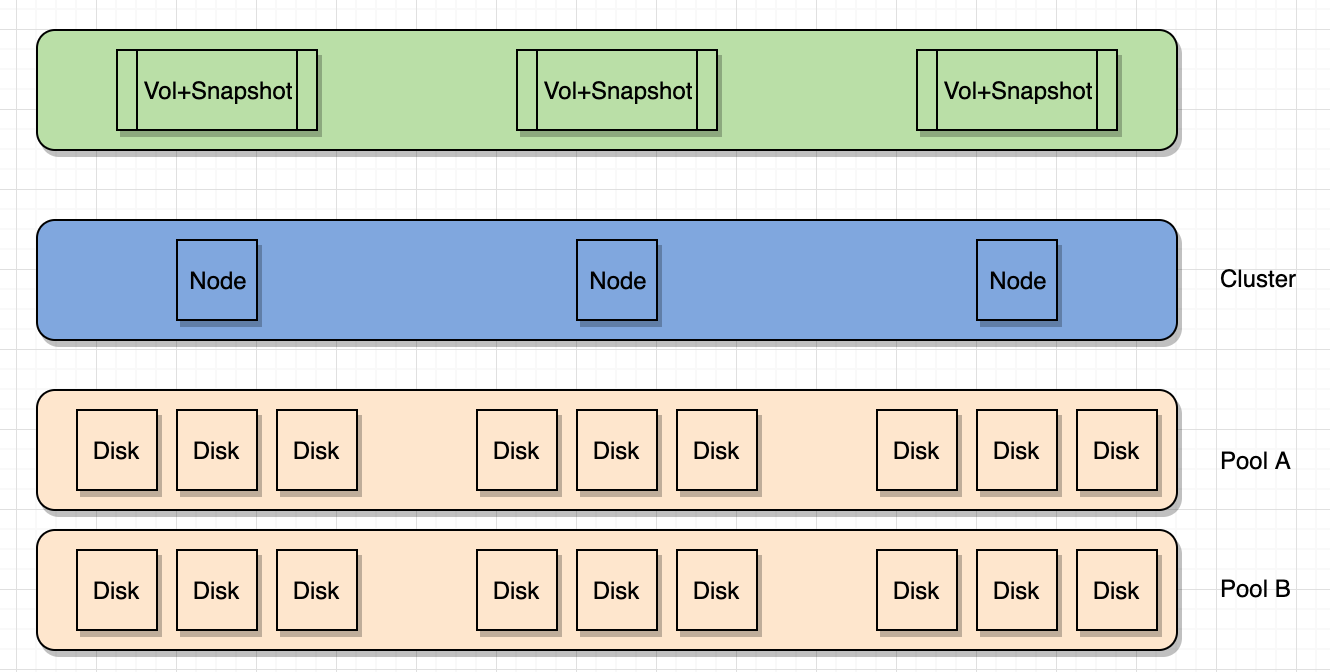
\includegraphics[width=0.8\textwidth]{../imgs/cluster-virt.png}
    \end{center}
\end{frame}

\begin{frame}[fragile]
    \frametitle{FusionStor的架构特点}
    \begin{myeasylist}{enumerate}
        & 元数据(非DHT)
        & 全用户态
        & core绑定 (PMD: polling mode driven)
        & Hugepage-based的内存管理
        & 直接访问裸盘(libaio/libnvme + KV)
        & 异步通信(TCP/RDMA)
        & 协议:iSCSI/iSER/NVMf
        & 编程模型:协程
    \end{myeasylist}
\end{frame}

\begin{frame}[fragile]
    \frametitle{从FusionStor到Suzaku}
    \begin{myeasylist}{enumerate}
        & 支持大卷
        & 单卷负载均衡
        & IO路径上的数据转发
        & 全局负载均衡(disk and core)
        & 元数据服务器MdCtl
            && 卷的元数据(chunk的副本信息)
            && ROW快照的v2p映射
        & KVDB
            && 副本位置信息
        & 更多信息记录在ETCD上
            && EFS ( +xattr )
            && 卷的引导信息
            && snapshot tree
    \end{myeasylist}
\end{frame}

\begin{frame}[fragile]
    \frametitle{Universal Flash Planform}
    \begin{center}
        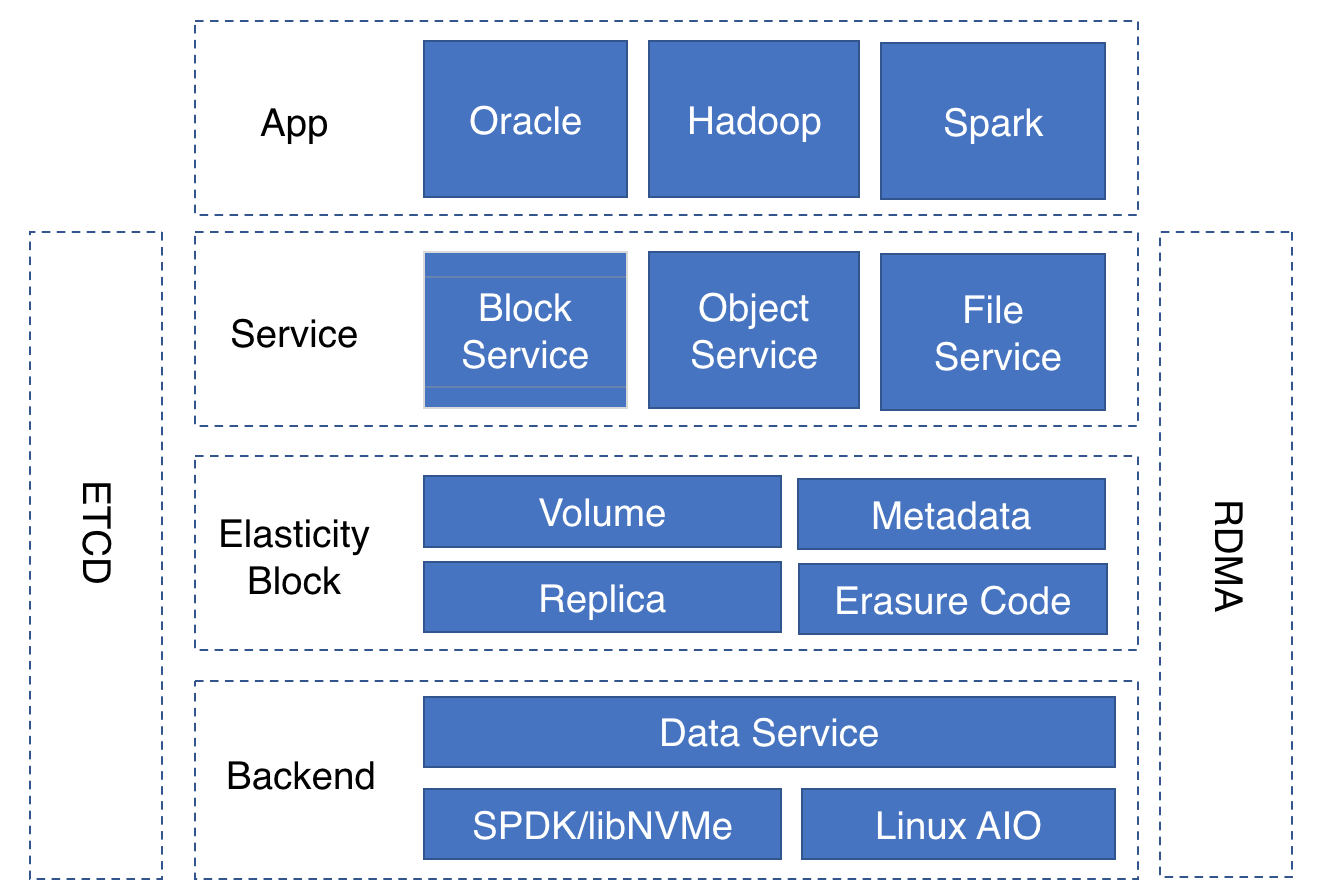
\includegraphics[width=0.6\textwidth]{../imgs/universal-flash.png}
    \end{center}
\end{frame}

\begin{frame}[fragile]
    \frametitle{操作系统}
    \begin{center}
        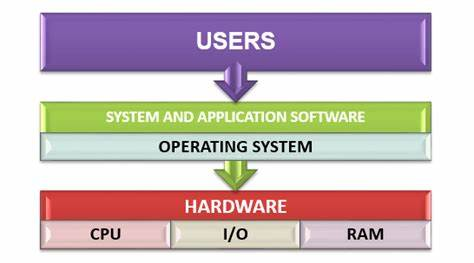
\includegraphics[width=0.5\textwidth]{../imgs/operating-system.jpeg}
    \end{center}
\end{frame}

\subsection{组件}

\begin{frame}[fragile]
    \frametitle{组件分解}
    \begin{columns}
        \begin{column}{0.5\textwidth}
            \begin{center}
                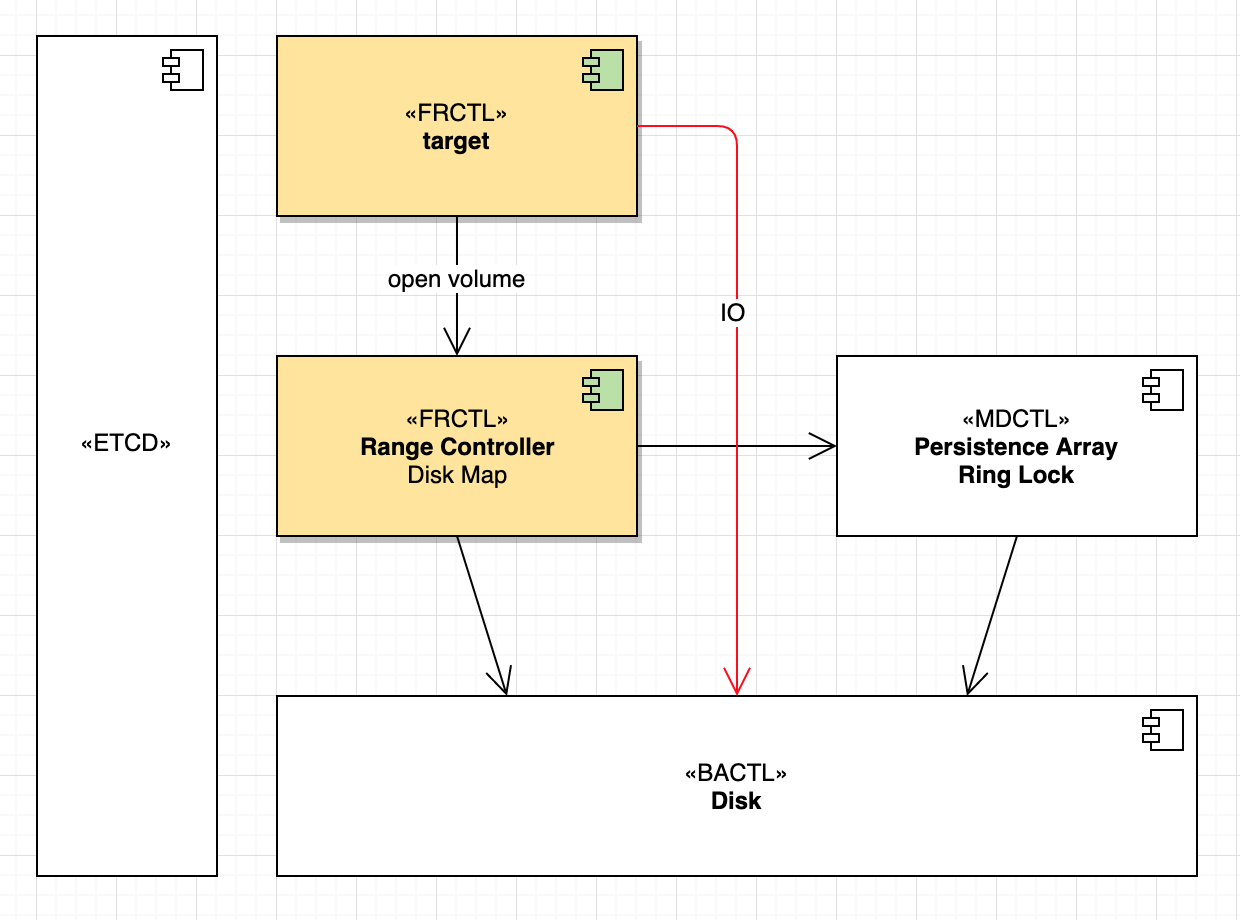
\includegraphics[width=0.9\textwidth]{../imgs/modules.png}
            \end{center}
        \end{column}

        \begin{column}{0.5\textwidth}
            \begin{center}
                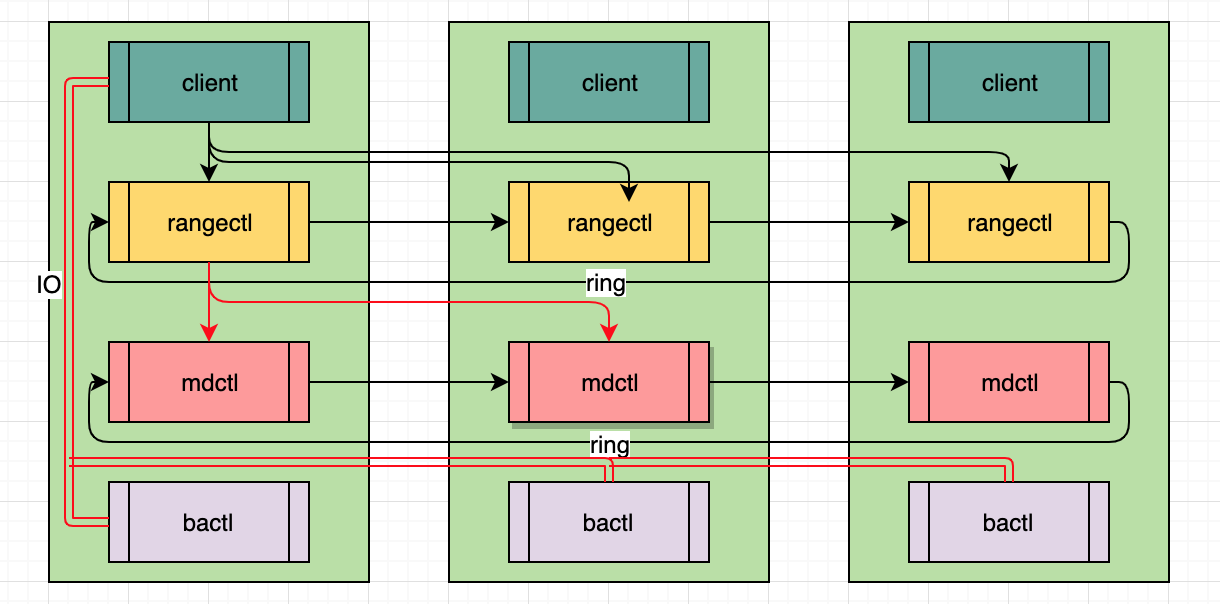
\includegraphics[width=0.9\textwidth]{../imgs/message-flow.png}
            \end{center}
        \end{column}
    \end{columns}

    \begin{myeasylist}{itemize}
        & Client
        & TgtCtl
        & FrCtl 
        & RangeCtl(VolumeCtl)
        & BaCtl
        & MdCtl
        & PoliCtl
    \end{myeasylist}
\end{frame}

\begin{frame}[fragile]
    \frametitle{卷的地址空间}
    \begin{center}
        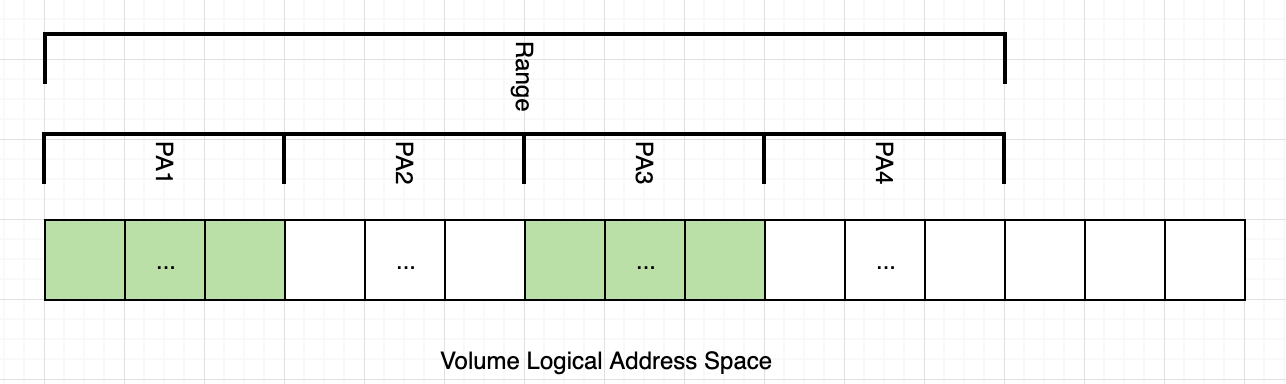
\includegraphics[width=0.9\textwidth]{../imgs/volume-addressspace.png}
    \end{center}

    \Activate
    \begin{tcolorbox}[title=分段管理]
        \begin{easylist}[itemize]
            & 一个卷包含若干range
            & 一个range包含1个Chunk(4M)
            & 估算卷的最大大小:4M/128 x 4M/128 x 4M = 4PB
        \end{easylist}
    \end{tcolorbox}
    \Deactivate
\end{frame}

\begin{frame}
    \frametitle{卷的元数据}
    \begin{center}
        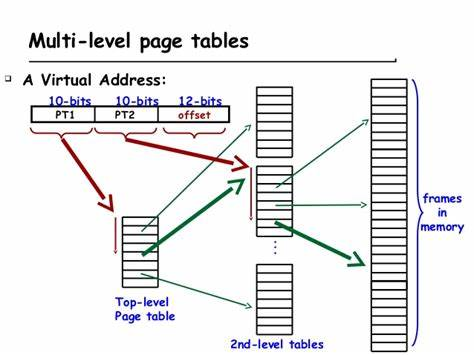
\includegraphics[width=0.6\textwidth]{../imgs/pagetable.jpeg}
    \end{center}
\end{frame}

\begin{frame}
    \frametitle{IO路径}
    \begin{center}
        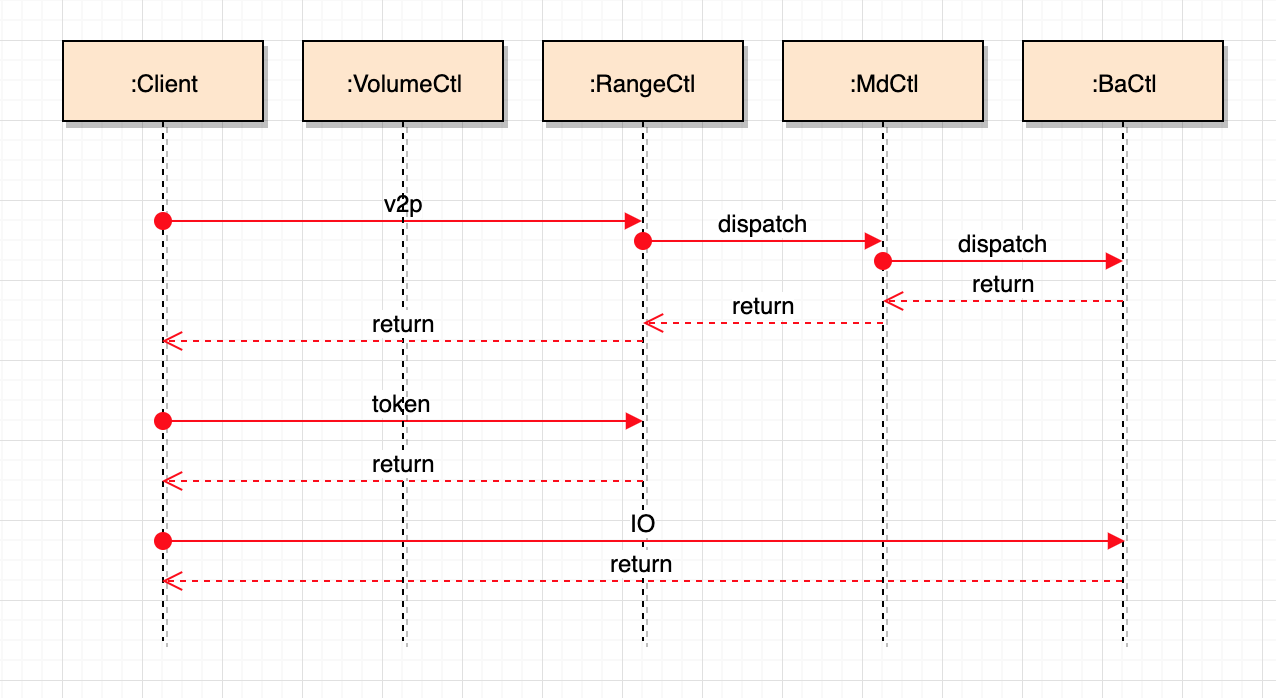
\includegraphics[width=0.9\textwidth]{../imgs/data-path.png}
    \end{center}
\end{frame}

\section{OS}

\subsection{CPU}

\begin{frame}[fragile]
    \frametitle{Event Framework}

    \begin{myeasylist}{itemize}
        & channel
    \end{myeasylist}
\end{frame}

\subsection{Memory}

\begin{frame}[fragile]
    \frametitle{Event Framework}

    \begin{myeasylist}{itemize}
        & hugepages
            && mem ring (ltgbuf\_t buddy-based)
            && vclock
            && spdk nvme driver
        & malloc
            && slab
    \end{myeasylist}
\end{frame}

\subsection{Disk}

\subsection{Network}

\section{配置}

\begin{frame}[fragile]
    \frametitle{配置coremask}
    \begin{center}
        \includegraphics[width=0.6\textwidth]{../imgs/coremask.png}
    \end{center}

    \begin{myeasylist}{itemize}
        & 根据测试结果进行增减
    \end{myeasylist}
\end{frame}

\section{快照}

\subsection{分析}

\begin{frame}[fragile]
    \frametitle{快照树}
    \begin{center}
        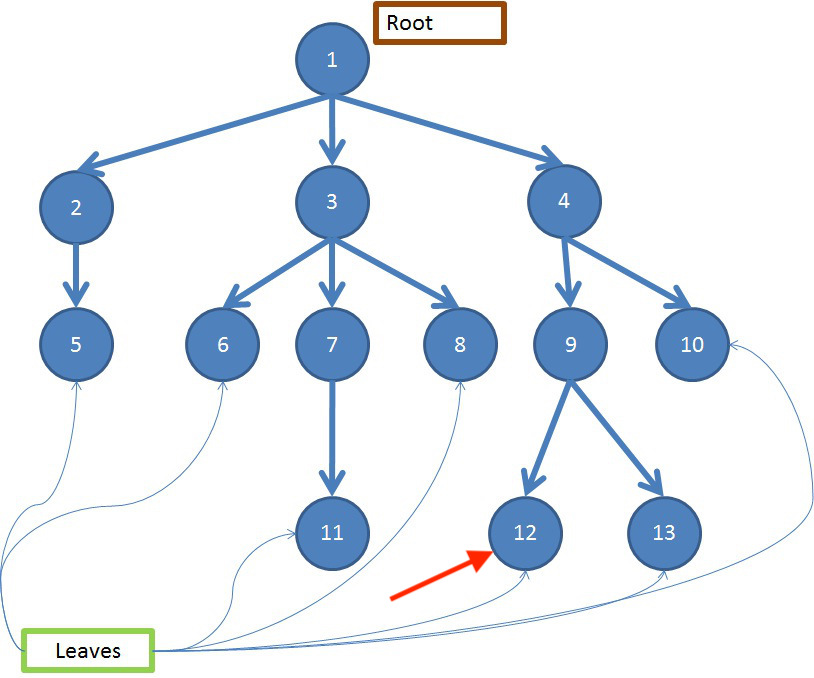
\includegraphics[width=0.6\textwidth]{../imgs/tree-data-structure.jpg}
    \end{center}
\end{frame}

\begin{frame}[fragile]
    \frametitle{操作复杂度分析}
    \Activate
    \begin{tcolorbox}[title=快照操作]
    \begin{easylist}[itemize]
        & create
        & delete
        & revert to
        & list
        & read
        & clone
        & flatten
        & protect/unprotect
    \end{easylist}
    \end{tcolorbox}
    \Deactivate

    \Activate
    \begin{tcolorbox}[title=IO操作 -- 快照和克隆改变了IO路径]
    \begin{easylist}[itemize]
        & write
        & read
    \end{easylist}
    \end{tcolorbox}
    \Deactivate
\end{frame}

\begin{frame}[fragile]
    \frametitle{评价指标}
    \begin{center}
        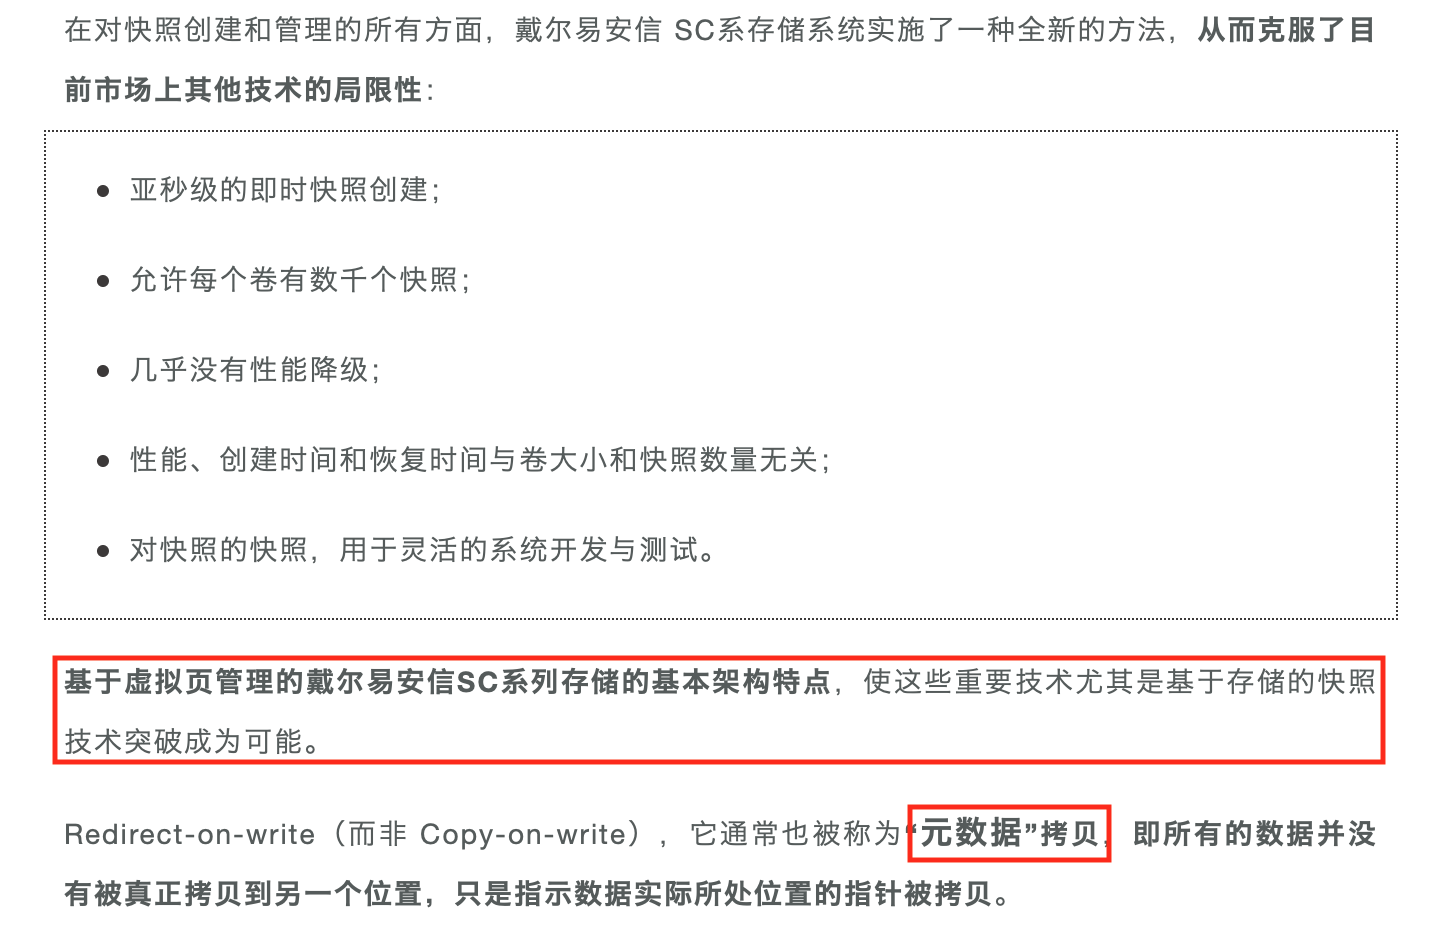
\includegraphics[width=0.8\textwidth]{../imgs/row-indexes.png}
    \end{center}
\end{frame}

\begin{frame}[fragile]
    \frametitle{COW}
    \begin{center}
        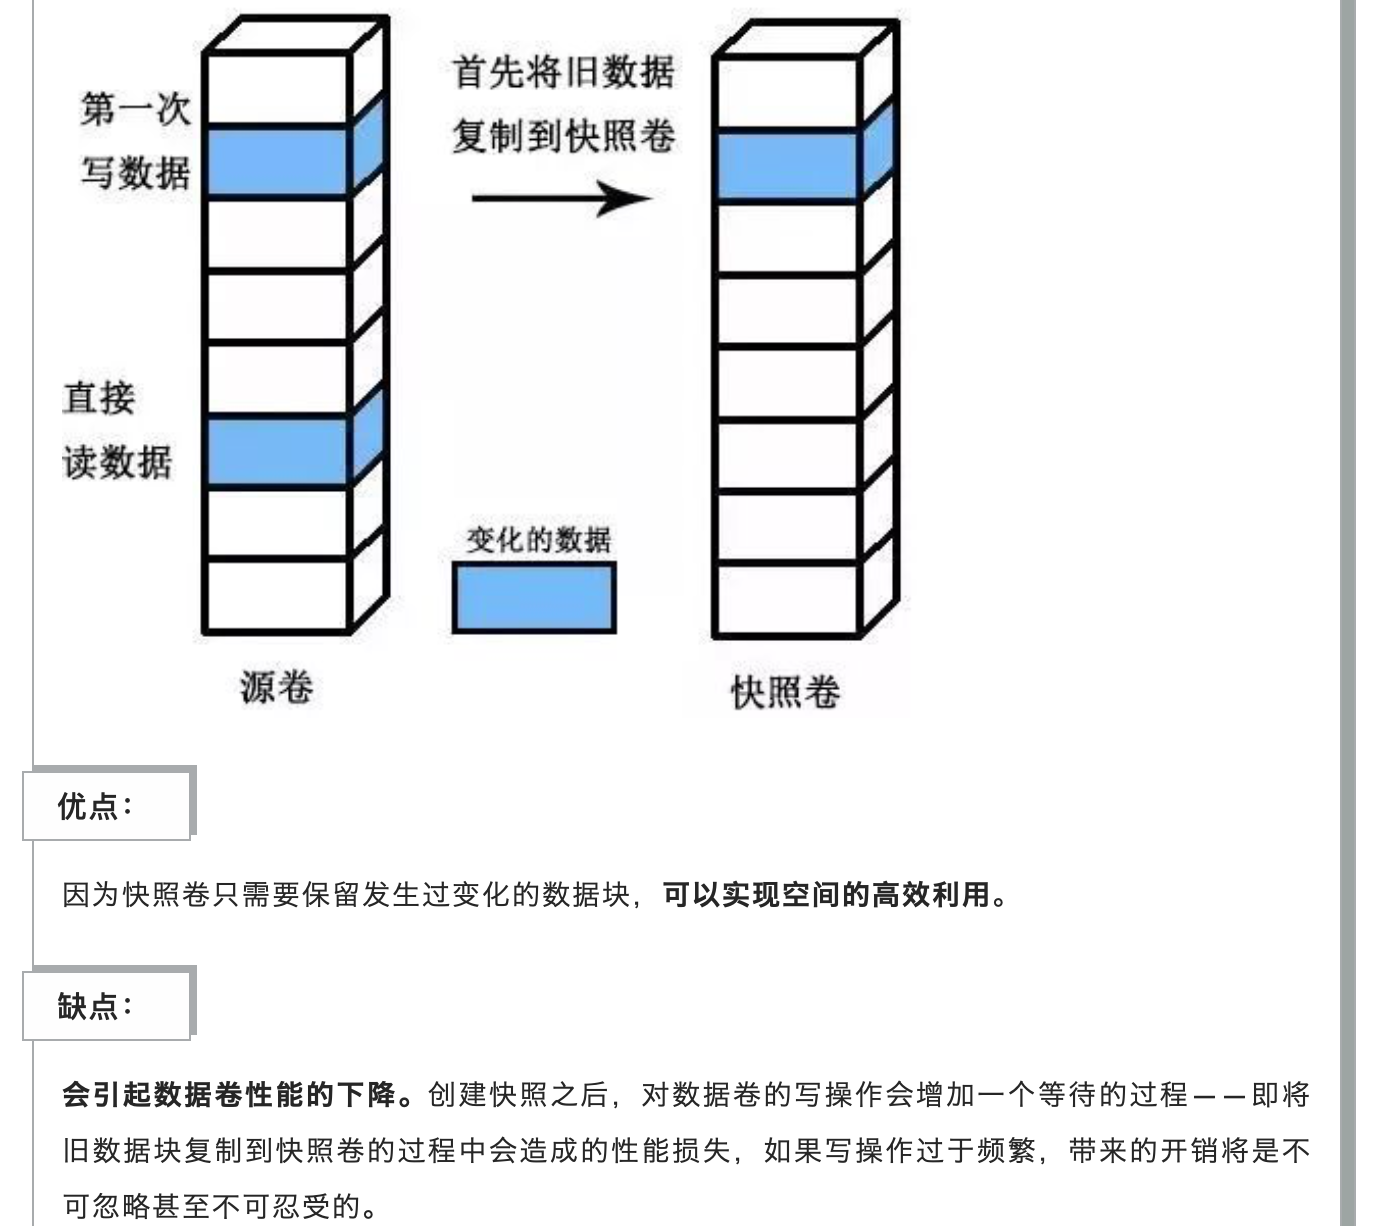
\includegraphics[width=0.6\textwidth]{../imgs/cow-snapshot.png}
    \end{center}
\end{frame}

\begin{frame}[fragile]
    \frametitle{ROW}
    \begin{center}
        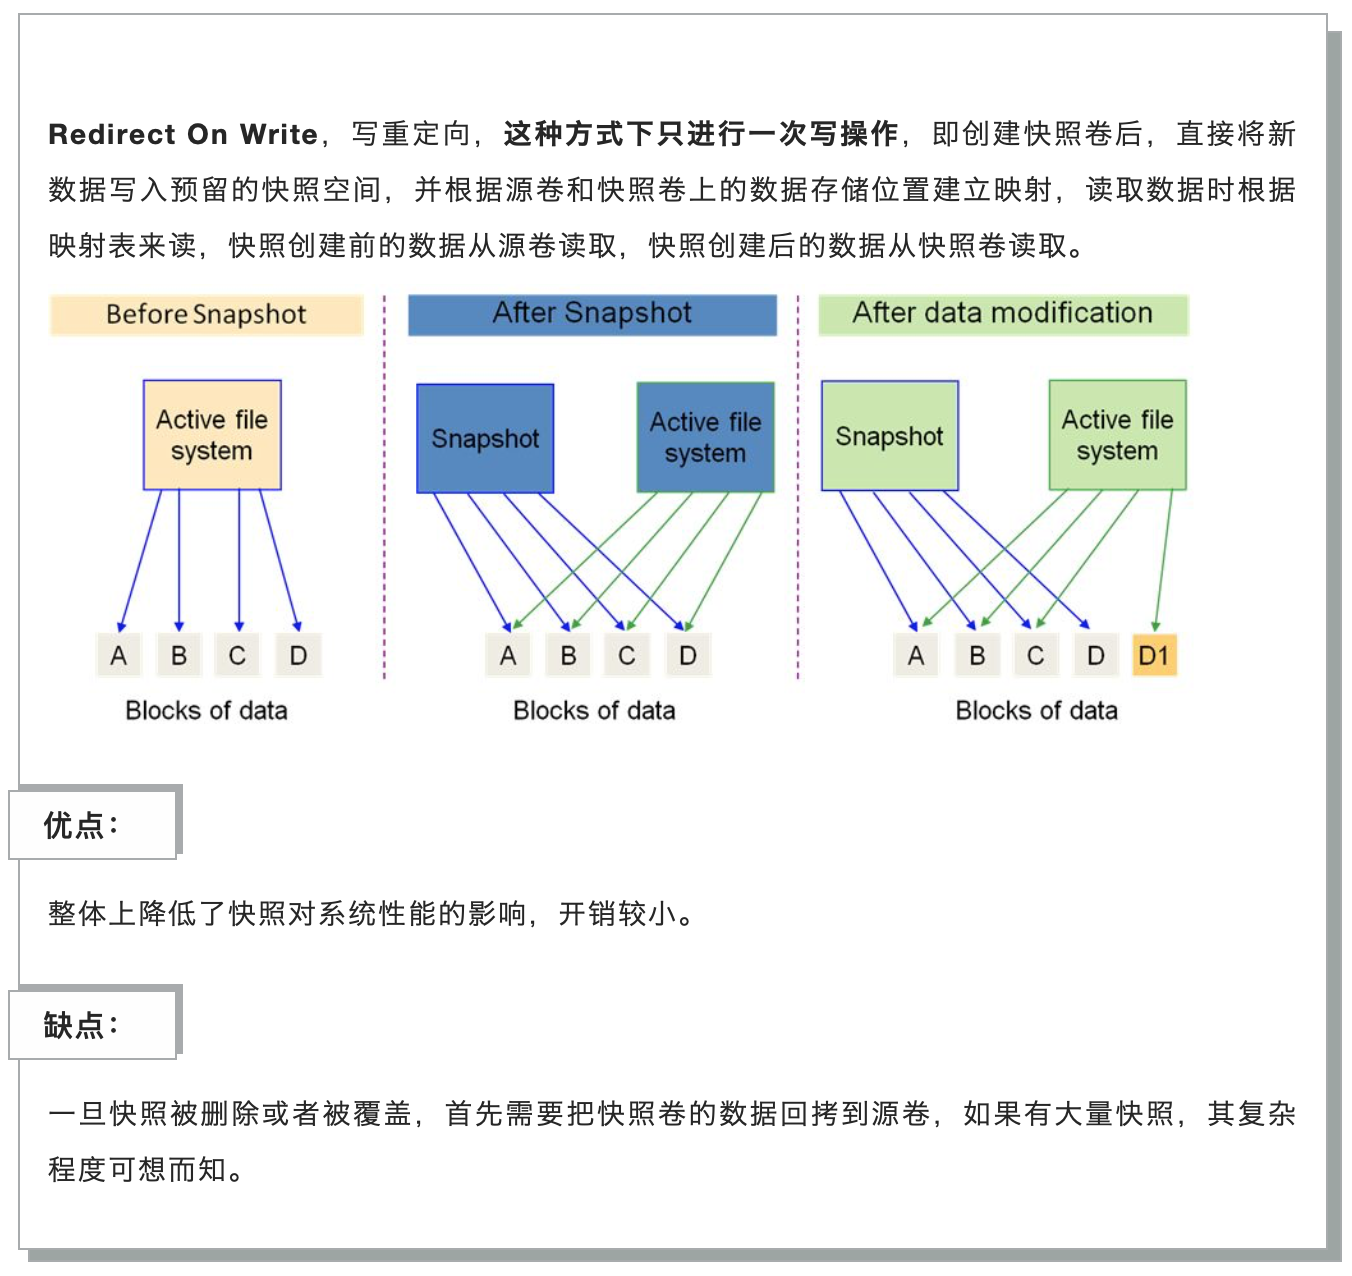
\includegraphics[width=0.6\textwidth]{../imgs/row-snapshot.png}
    \end{center}
\end{frame}

\begin{frame}[fragile]
    \frametitle{日志系统}
    \begin{center}
        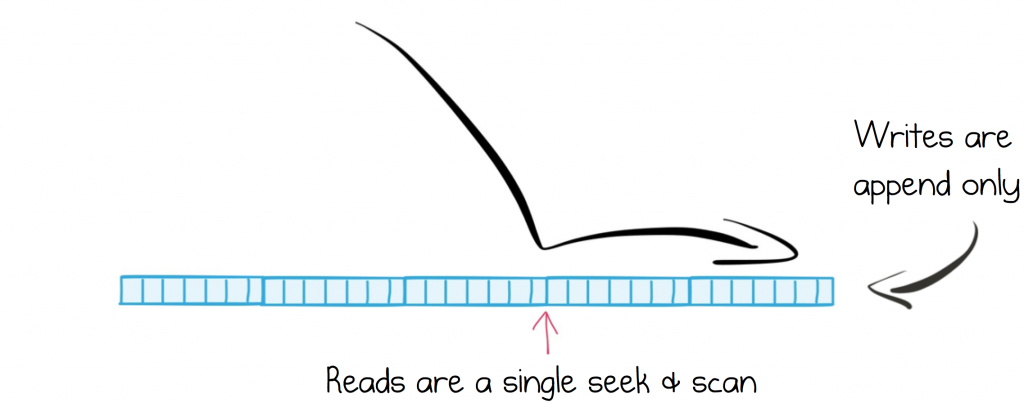
\includegraphics[width=0.8\textwidth]{../imgs/log-structured.png}
    \end{center}
\end{frame}

\begin{frame}[fragile]
    \frametitle{COW or ROW}
    \begin{center}
        
\includegraphics[width=0.4\textwidth]{../imgs/question-mark.jpg}
    \end{center}
\end{frame}

\subsection{实现}

\begin{frame}[fragile]
    \frametitle{引入新的卷格式}
    \begin{center}
        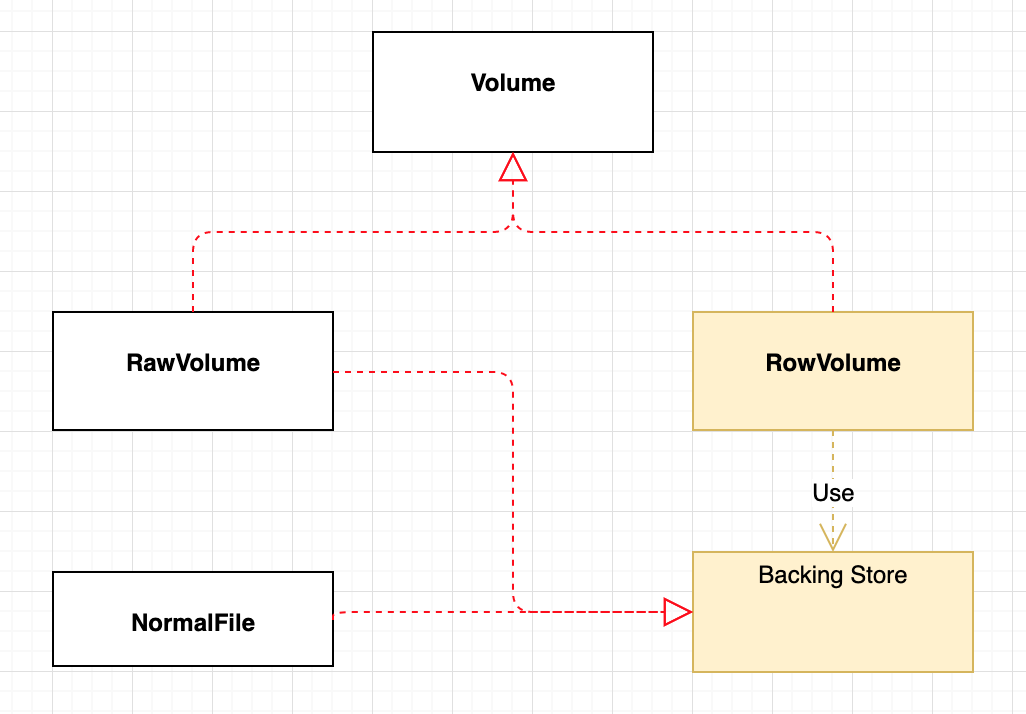
\includegraphics[width=0.4\textwidth]{../imgs/volume-type.png}
    \end{center}
    \begin{myeasylist}{itemize}
        & 创建卷时,指定RAW或ROW格式
        & 在哪一层实现ROW? (RAW卷之上或之下)
        & 虚拟卷和物理卷的关系(1:1, 1: m)
        & 卷ID保持不变
        & 元数据的粒度:chunk or page
        & 如何支持比4K更小的IO,如512B?
        & CHUNK内append模式,避免随机写浪费空间
        & 底层空间allocator,负责分配和释放CHUNK,以及策略
        & 没有快照时,IO路径如何?
    \end{myeasylist}
\end{frame}

\begin{frame}[fragile]
    \frametitle{卷的虚拟ID}

    \begin{center}
        \includegraphics[width=0.6\textwidth]{../imgs/row/row-changed-id.png}
    \end{center}

    \begin{myeasylist}{itemize}
        & 创建快照后,生成新卷,定义为\hl{当前可写快照}
        & 引入不变的虚拟ID以实现透明性
        & \hl{rangectl上利用卷的快照树信息映射虚拟id到当前快照}
        & 相关(use virtual volume id)
            && EFS结构
            && volume open
    \end{myeasylist}
\end{frame}

\begin{frame}[fragile]
    \frametitle{ROW卷的数据布局}
    \begin{center}
        \includegraphics[width=0.6\textwidth]{../imgs/row/row-data-layout.png}
    \end{center}

    \begin{myeasylist}{itemize}
        & bitmap记录每页数据所在位置,满足引用一致性条件
        & 按range分段管理bitmap
        & 采用事务机制
    \end{myeasylist}
\end{frame}

\begin{frame}[fragile]
    \frametitle{管理range bitmap}
    \begin{center}
        \includegraphics[width=0.6\textwidth]{../imgs/row/row-bitmap.png}
    \end{center}

    \begin{myeasylist}{itemize}
        & v2p过程区分real/user range size
        & 每个range的bitmap cache按页组织 (array, flag跟踪dirty)
        & range内chunk个数:127G/4M = 32512
        & 每个4M slice需要2 bitmap pages,故所需bitmap page个数:65024
    \end{myeasylist}
\end{frame}

\begin{frame}[fragile]
    \frametitle{ROW卷的allocate和IO}

    \begin{myeasylist}{itemize}
        & 所有io都通过bitmap定位
        & 所以allocate也要填充bitmap
        & 先写入数据,后更新bitmap,注意满足ACID条件
        & 分页IO
            && 页alignment (首页-中间页-尾页)
            && RMW
            && 按页读,按页写
            && batch模式(最大连续段)
    \end{myeasylist}
\end{frame}

\begin{frame}[fragile]
    \frametitle{创建快照后ROW卷的allocate和IO}

    \begin{myeasylist}{itemize}
        & 创建快照后,生成新卷,原卷变成只读快照,新卷复制元数据(COW,读的时候也要复制?)
        & get token时传入io参数(返回一个或多个记录,可能引用到另外的slice)
        & 碎片化
        & 优化
    \end{myeasylist}
\end{frame}

\begin{frame}[fragile]
    \frametitle{ROW卷的数据布局}
    \begin{center}
        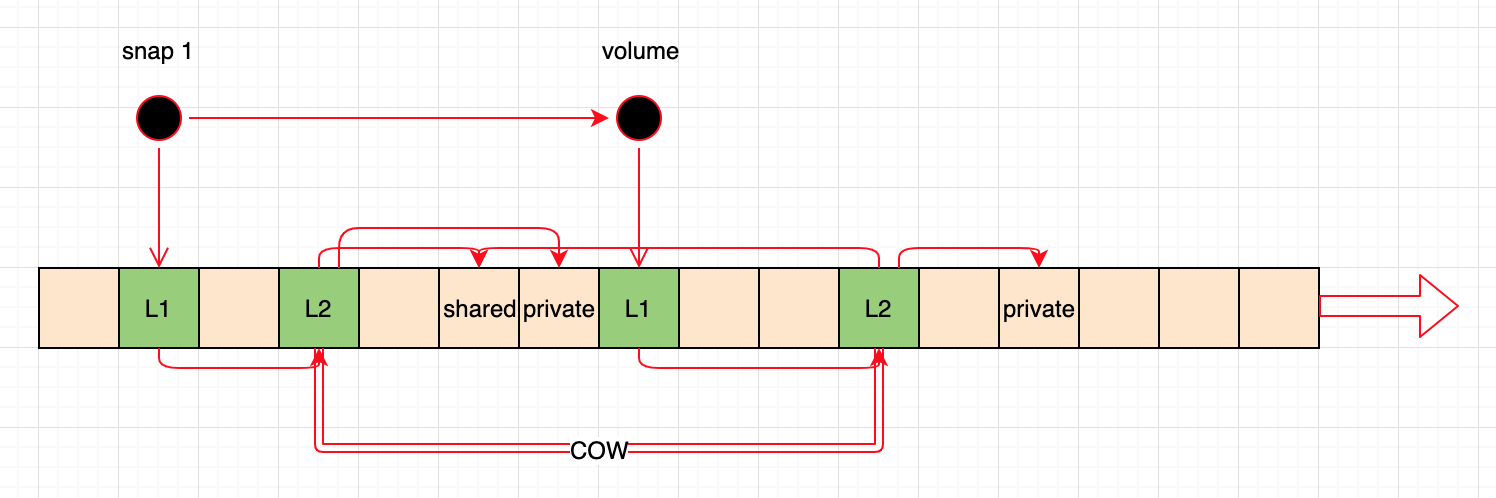
\includegraphics[width=0.9\textwidth]{../imgs/row-layout.png}
    \end{center}

    \begin{myeasylist}{itemize}
        & 一个快照头可以拥有多个L1 chunk,以支持扩展
        & 跟踪L2 chunk和RAW chunk的ownership关系
            && 发生COW的L2 chunk即为私有
            && 发生write的RAW chunk即为私有
    \end{myeasylist}
\end{frame}

\begin{frame}[fragile]
    \frametitle{从逻辑地址到物理地址}
    \begin{columns}
        \begin{column}{0.4\textwidth}
            \begin{center}
                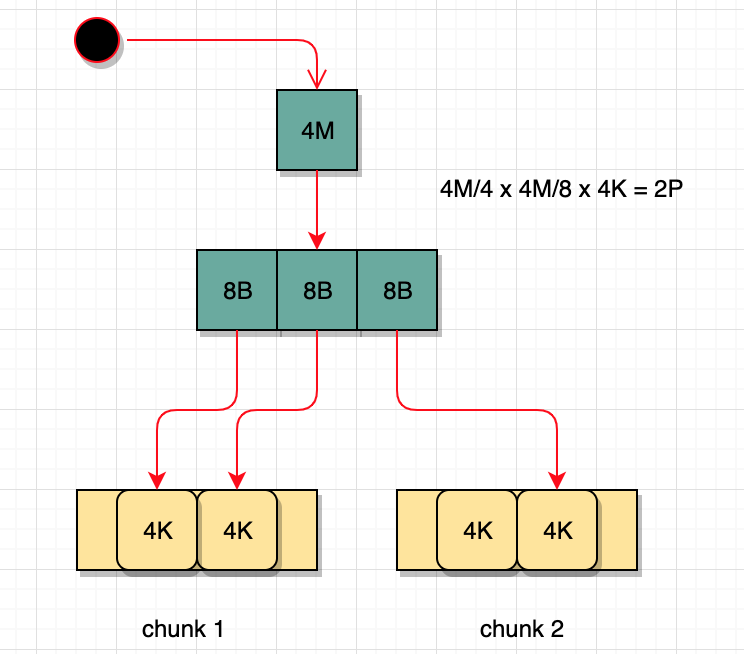
\includegraphics[width=0.9\textwidth]{../imgs/row-head.png}
            \end{center}
        \end{column}

        \begin{column}{0.4\textwidth}
            \begin{center}
                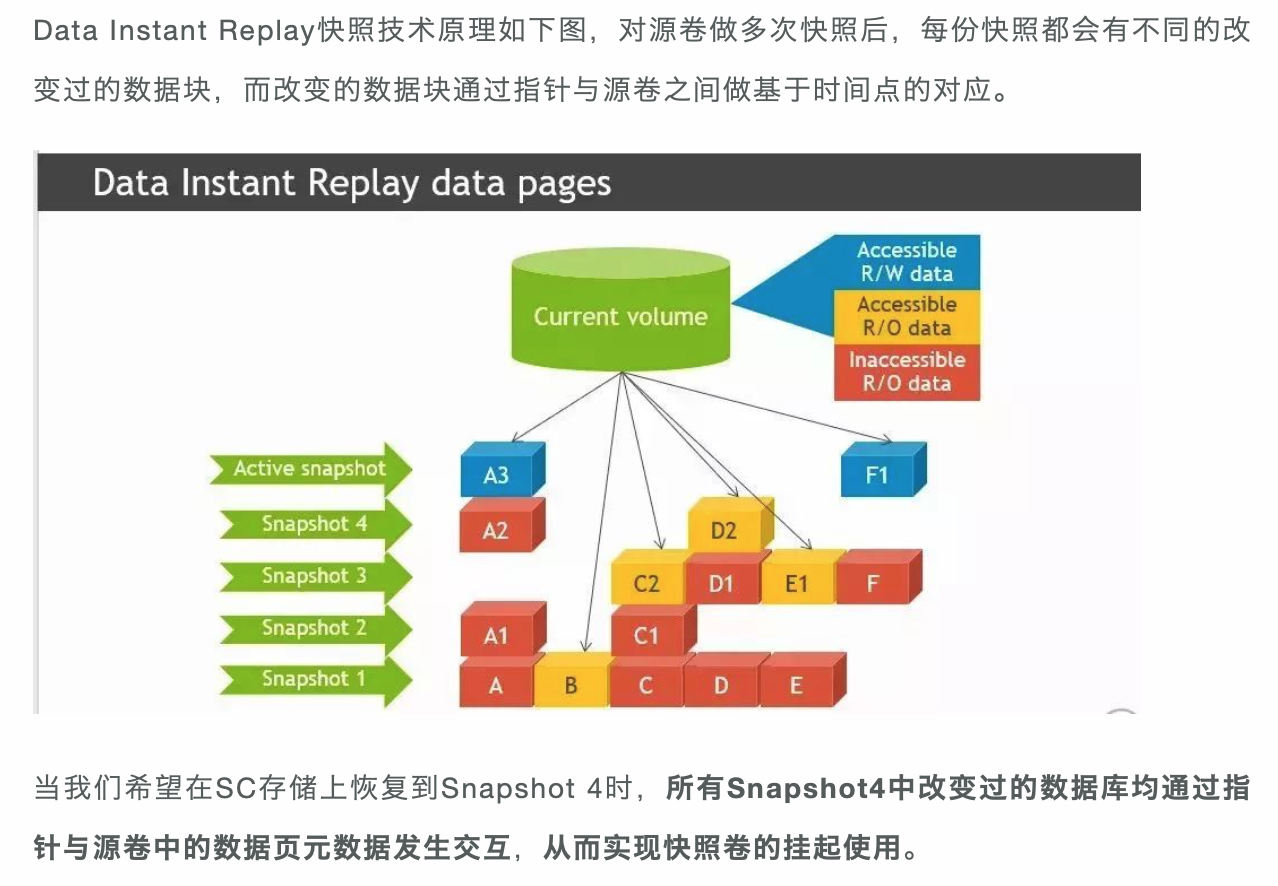
\includegraphics[width=0.9\textwidth]{../imgs/data-replay.png}
            \end{center}
        \end{column}
    \end{columns}

    \begin{myeasylist}{itemize}
        & 逻辑上连续的页,物理上未必连续
        & 全量索引,一跳即完成V2P映射
        & 每个快照都有快照头,卷可以看作是一个特殊快照(可写、当前)
        & 快照头包含两层元数据
        & \hl{V2P内置于get token过程},分为两步:
            && 选择正确的快照头
            && 根据快照头进行定位
    \end{myeasylist}
\end{frame}

\begin{frame}[fragile]
    \frametitle{引入VolumeCtl}
    \begin{myeasylist}{itemize}
        & 处理快照的创建、删除、revert等操作
        & 如何与IO路径进行协作?
            && VolumeCtl位于每个rangectl上
            && 采用2PL提交协议
    \end{myeasylist}
\end{frame}

\begin{frame}[fragile]
    \frametitle{创建快照}
    \begin{center}
        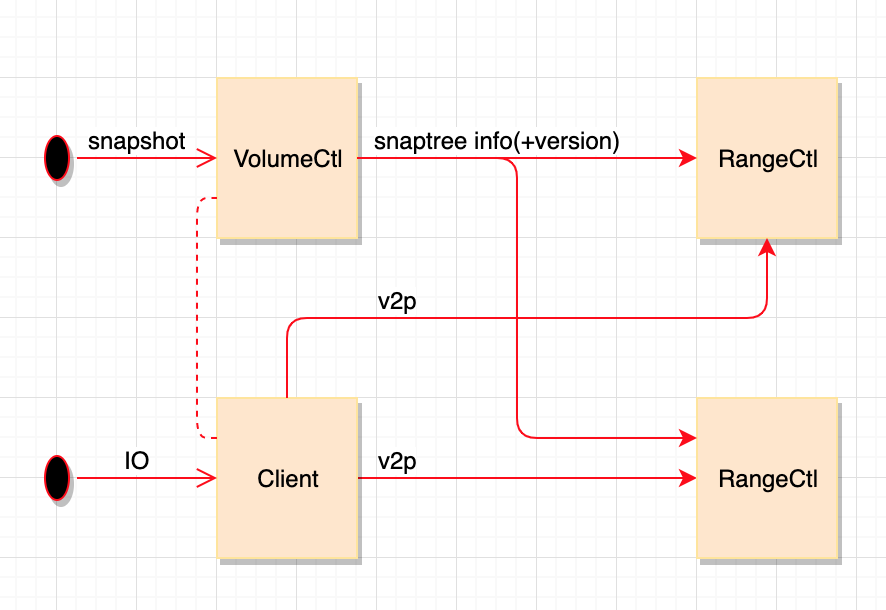
\includegraphics[width=0.6\textwidth]{../imgs/row-create.png}
    \end{center}

    \begin{columns}
        \begin{column}{0.5\textwidth}
            \Activate
            \begin{tcolorbox}[title=场景]
                \begin{easylist}[itemize]
                        & 跨Range IO
                \end{easylist}
            \end{tcolorbox}
            \Deactivate
        \end{column}
        \begin{column}{0.5\textwidth}
            \Activate
            \begin{tcolorbox}[title=RangeCtl看到同一快照树结构]
                \begin{easylist}[itemize]
                        & version
                        & publish-subscribe
                        & distributed lock
                        & others ...
                        & \hl{consistency group}, for RAC
                \end{easylist}
            \end{tcolorbox}
            \Deactivate
        \end{column}
    \end{columns}

\end{frame}

\begin{frame}[fragile]
    \frametitle{Crash Consistency}
    \begin{center}
        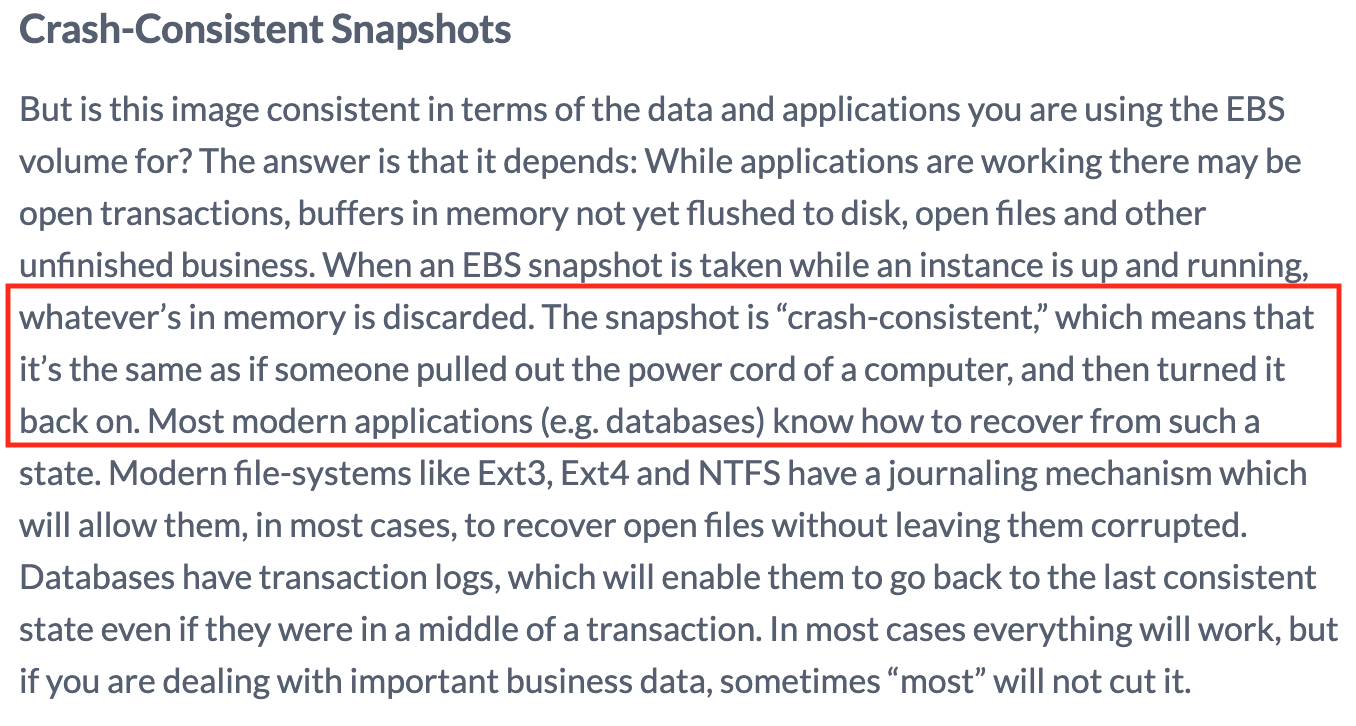
\includegraphics[width=0.8\textwidth]{../imgs/crash-consistency.png}
    \end{center}
\end{frame}

\begin{frame}[fragile]
    \frametitle{Application Consistency}
    \begin{center}
        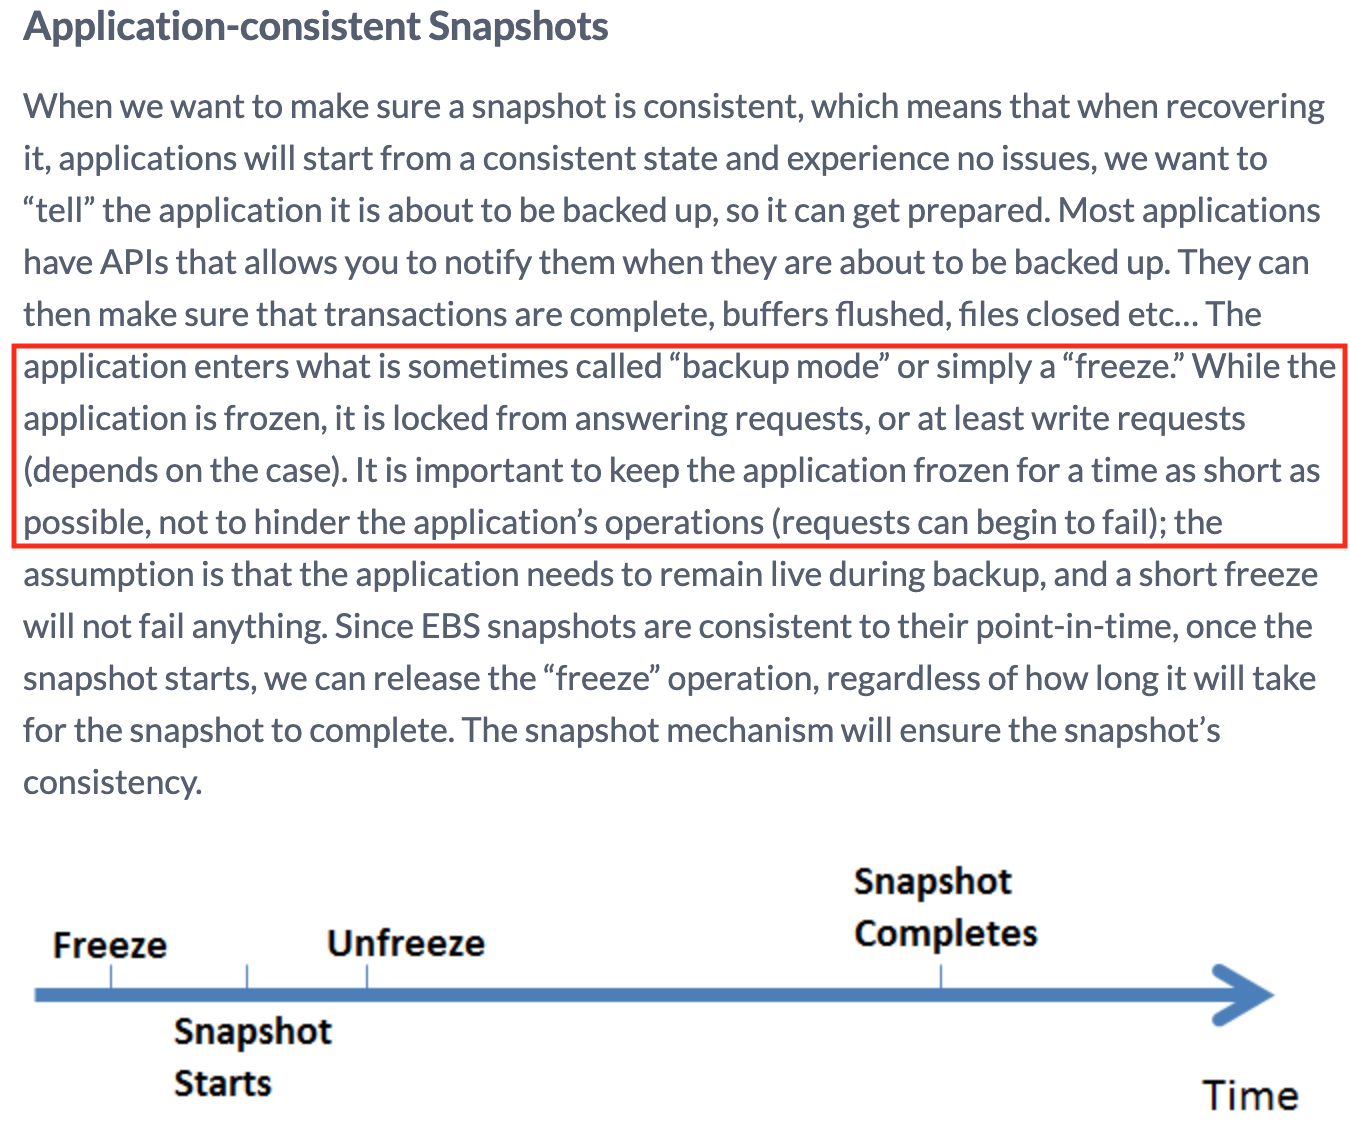
\includegraphics[width=0.8\textwidth]{../imgs/application-consistency.png}
    \end{center}
\end{frame}

\begin{frame}[fragile]
    \frametitle{删除快照}
    \begin{columns}
        \begin{column}{0.5\textwidth}
            \begin{center}
                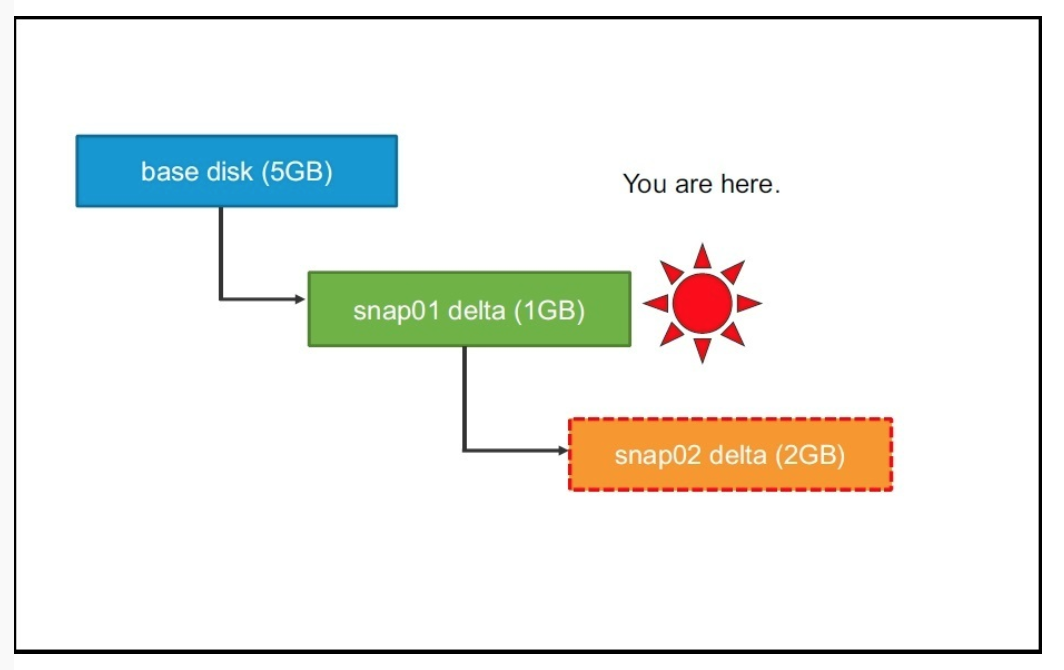
\includegraphics[width=1.0\textwidth]{../imgs/snap-delete-leaf.png}
            \end{center}
        \end{column}

        \begin{column}{0.5\textwidth}
            \begin{center}
                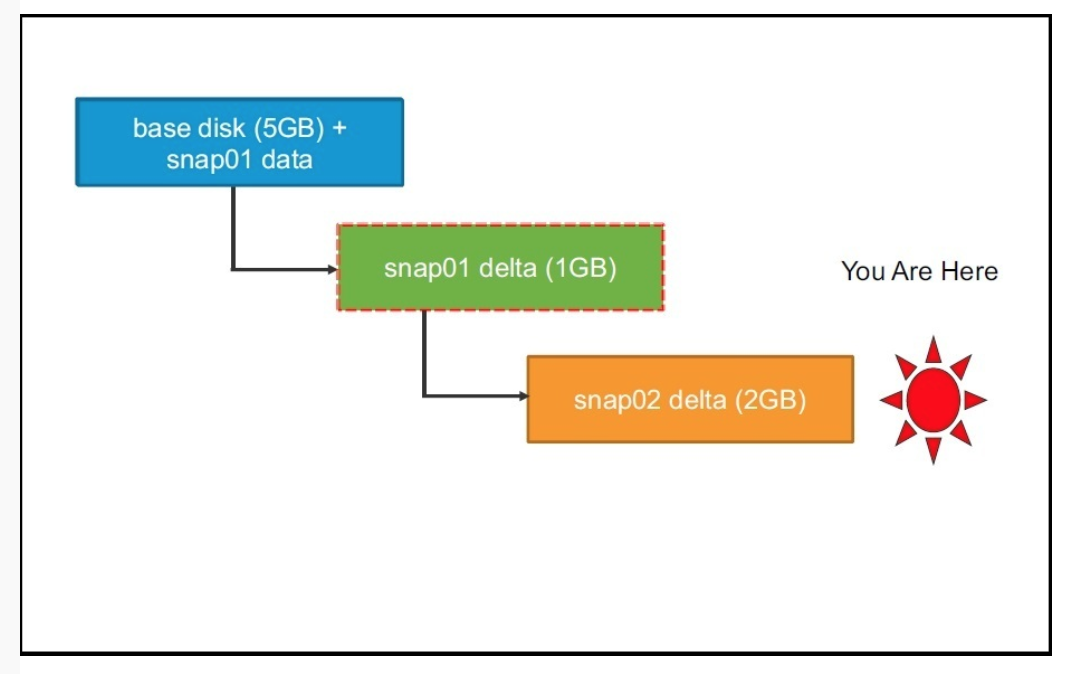
\includegraphics[width=1.0\textwidth]{../imgs/snap-delete-non-leaf.png}
            \end{center}
        \end{column}
    \end{columns}
    \begin{myeasylist}{itemize}
        & 先实现为标记删除(叶子节点可直接删除,中间节点仅仅做删除标记)
    \end{myeasylist}
\end{frame}

\begin{frame}[fragile]
    \frametitle{Revert to}
    \begin{center}
        \includegraphics[width=0.8\textwidth]{../imgs/revert.png}
    \end{center}

    \begin{myeasylist}{itemize}
        & 实现为快照树结构,revert操作后snap3依然有效
        & copy目标快照头,创建新的卷
        & 异步回收原卷的快照头及其私有数据
    \end{myeasylist}
\end{frame}

\begin{frame}[fragile]
    \frametitle{CLONE卷}
    \begin{center}
        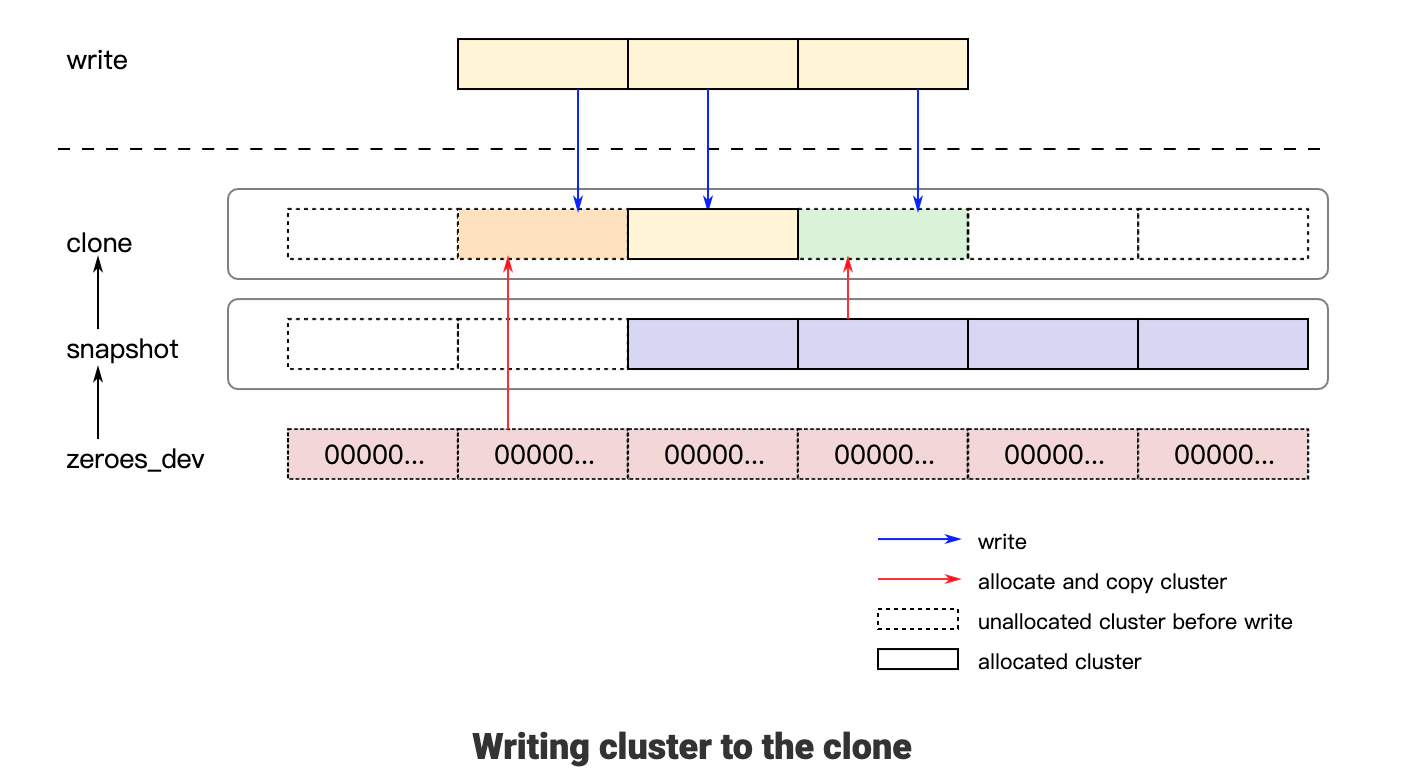
\includegraphics[width=0.8\textwidth]{../imgs/clone-write.png}
    \end{center}

    \begin{myeasylist}{itemize}
        & 透明性:clone卷使用上在与普通卷没有区别
            && 支持多阶clone
        & 通过分离操作,clone卷变成普通卷
    \end{myeasylist}
\end{frame}

\begin{frame}[fragile]
    \frametitle{CLONE卷}
    \begin{center}
        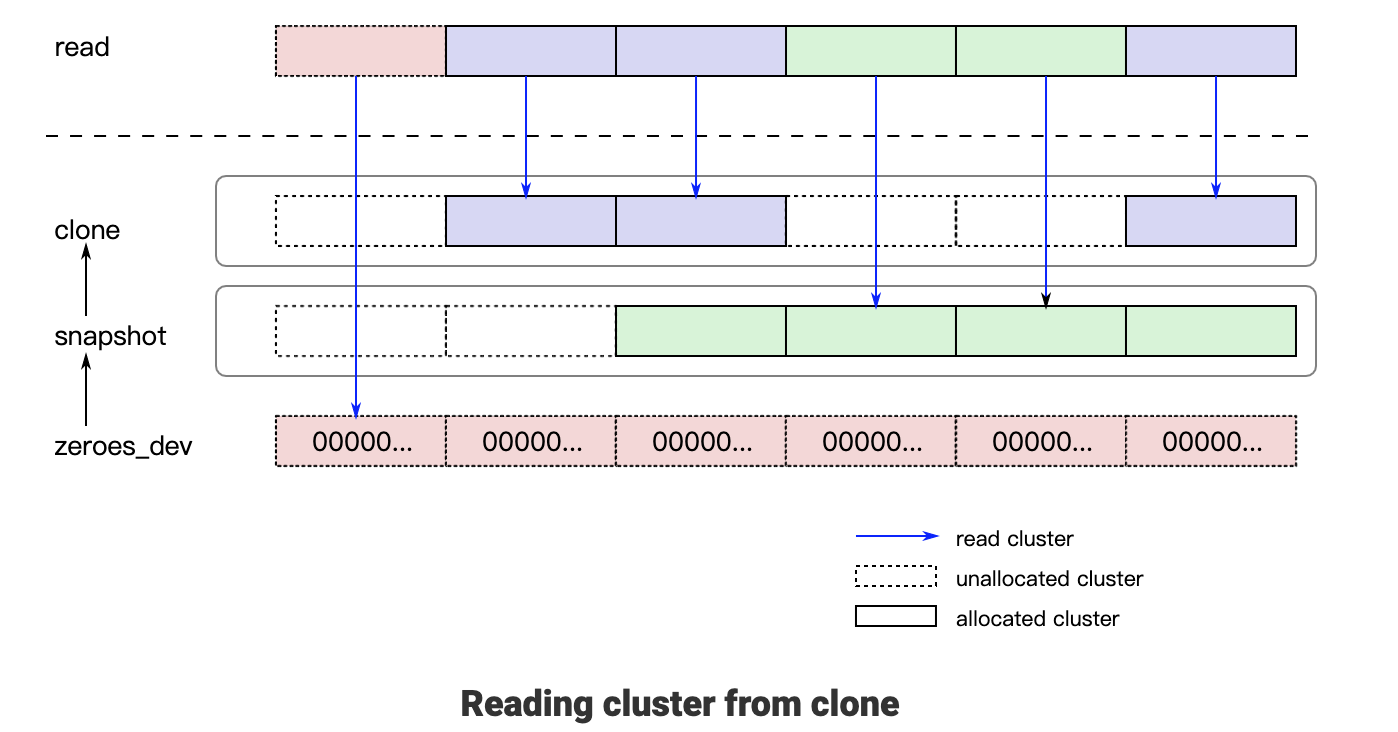
\includegraphics[width=0.8\textwidth]{../imgs/clone-read.png}
    \end{center}
\end{frame}

\begin{frame}[fragile]
    \frametitle{重点问题}
    \begin{myeasylist}{itemize}
        & ROW重点问题:
        && ROW卷ID会发生变化,影响到efs和io
        && 引入bitmap后,即相当于引入了一种卷格式
        && bitmap更新的事务处理
        && 支持多阶clone
        && 支持一致性快照组
        && 抽象快照卷相关接口,以支持多态行为
        & 可重用的部分:
        &&  快照树数据结构
        &&  2PL提交协议
        & 其它:
        &&  COW如何实现快照树
    \end{myeasylist}
\end{frame}

\subsection{参考}

\begin{frame}[fragile]
    \frametitle{参考产品}
    \begin{myeasylist}{itemize}
            & 阿里云ECS
            & 华为FusionStorage
            & DELL SC Series
            & VMWare
            % & NetApp WALFS
            & SSAN
            & Open Vstorage
            & QEMU qcow2
            & SPDK
    \end{myeasylist}
\end{frame}

\section{一致性}

\begin{frame}[fragile]
    \frametitle{一致性分割}
    \begin{center}
        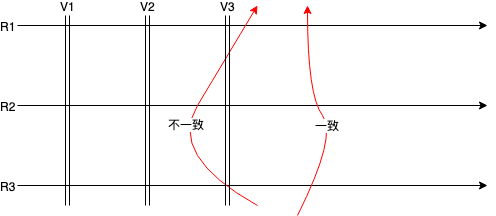
\includegraphics[width=0.6\textwidth]{../imgs/consistency-splice.png}
    \end{center}

    \begin{columns}
        \begin{column}{0.5\textwidth}
            \Activate
            \begin{tcolorbox}[title=规定]
                \begin{easylist}[itemize]
                    & 更新一致性
                    & 读取一致性
                    & 副本一致性
                    & EC一致性
                \end{easylist}
            \end{tcolorbox}
            \Deactivate
        \end{column}
        \begin{column}{0.5\textwidth}
            \Activate
            \begin{tcolorbox}[title=实现]
                \begin{easylist}[itemize]
                    & Leader
                    & Version
                    & Journal
                \end{easylist}
            \end{tcolorbox}
            \Deactivate
        \end{column}
    \end{columns}
\end{frame}

\begin{frame}[fragile]
    \frametitle{一致性实现}

    \begin{myeasylist}{itemize}
        & 强一致性
            && 各副本按相同顺序写入
            && 成功提交的数据不丢失
            && read last committed
        & 异步修复
            && mark dirty
            && degrade mode
    \end{myeasylist}

    \begin{myeasylist}{itemize}
        & Tgtctl的唯一性
            && Session安全
        & RangeCtl的唯一性
            && Slice状态机
        & 副本
            && vclock保序
    \end{myeasylist}
\end{frame}

\section{性能}

\begin{frame}[fragile]
    \frametitle{平衡过程}
    \begin{center}
        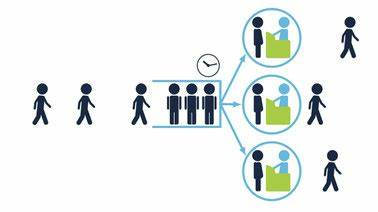
\includegraphics[width=0.6\textwidth]{../imgs/queuing.jpeg}
    \end{center}

    \begin{myeasylist}{itemize}
        & 流出量和流入量趋于平衡
        & 流入量 \ding{226} 调度能力 \ding{226} 处理能力
    \end{myeasylist}
\end{frame}

\section{FAQ}

% \subsection{Session}

\begin{frame}[fragile]
    \frametitle{什么是session}

    \begin{myeasylist}{itemize}
        & 参考RFC 3720
        & session管理不善,会导致数据一致性问题
    \end{myeasylist}
\end{frame}

% \subsection{IO TOKEN}

\begin{frame}[fragile]
    \frametitle{什么是token}

    \begin{myeasylist}{itemize}
        & 实现io保序的机制
    \end{myeasylist}
\end{frame}

\end{document}
